%----------------------------------------------------------------------------------------
%	PACKAGES AND DOCUMENT CONFIGURATIONS
%----------------------------------------------------------------------------------------
\documentclass[a4paper, 12pt]{article}

%\documentclass{article}

\usepackage{graphicx} % Required for the inclusion of images
\usepackage{natbib} % Required to change bibliography style to APA
\usepackage{amsmath} % Required for some math elements 

\setlength\parindent{0pt} % Removes all indentation from paragraphs

\renewcommand{\labelenumi}{\alph{enumi}.} % Make numbering in the enumerate environment by letter rather than number (e.g. section 6)

%\usepackage{times} % Uncomment to use the Times New Roman font


%\usepackage[latin1]{inputenc}

\usepackage{amsmath, amssymb}

\usepackage[finnish]{babel}
\usepackage[utf8x]{inputenc}
\usepackage{fancyhdr}
\usepackage{listings}


\usepackage{listings}
\usepackage{color}

\usepackage{graphicx}
\usepackage{hyperref}
\usepackage{wrapfig}
\usepackage{lscape}
\usepackage{rotating}
\usepackage{epstopdf}

\lstset{ %
  backgroundcolor=\color{white},
  basicstyle=\footnotesize,
  language=Java,
  tabsize=2
}

%----------------------------------------------------------------------------------------
%	DOCUMENT INFORMATION
%----------------------------------------------------------------------------------------

\title{Säteilyn ilmaisin} % Title

\author{Alexey \textsc{Sofiev}} % Author name

\date{\today} % Date for the report

\begin{document}

\maketitle % Insert the title, author and date

\begin{center}
\begin{tabular}{l r}
Suorituspäivä: & 18 Toukokuuta, 2016 \\ % Date the experiment was performed
Työpari: & Tudor Florea \\ % Partner names
& Jari Honko \\
Opiskelijanumeroni: & 013573003 % Instructor/supervisor
\end{tabular}
\end{center}

\clearpage
\section{Tiivistelmä}

Fysiikan aineopintojen toisen laboratoriotyön tarkoituksena oli rakentaa tuikeilmaisin havaitakseen gammasäteilyä. Päätehtävänä oli tutustua tuikeilmaisimen toimintaan ja siinä hyödynnettävään elektroniikkaan. Lisätehtävänä oli tutkia säteilyn vaimenemista lyijyssä.

\clearpage

\section{Johdanto}

Tämän laboratoriotyön tarkoituksena oli rakentaa laitteisto, joka pystyisi havaitsemaan gammasäteilyä. Työssä ollaan valittu tuikekide havainnointikappaleeksi, joka muuntaa osuvaa gammasäteilyä valon tuikahdukseksi. Saatu signaali on kuitenkin hieman heikko, joten ennen sen rekisteröintiä se päästetään valomonistinputkesta läpi (PMT, photomultiplier tube), jonka jälkeen voimistunut valosignaali kerätään ja muutetaan sähköiseksi signaaliksi. Muuttaminen tapahtuu esivahvistimen avulla. Saatu signaali ohjataan tietokoneen äänikortille, josta se kerätään talteen PRA11 ohjelman avulla.

Ennen varsinaista mittausta tutkitiin rakennetun piirin ulostulevan signaalin muotoja oskilloskoopilla, mm. esivahvistin ja vahvistin.

Mittaukset aloitettiin taustasäteilyn mittauksella, jotta sitä voitais poistaa analyysivaiheessa. Säteilyn lähteenä oli Cs-137, ja se oli asetettu parin cm korkeudelle lähteestä. Gammasäteilyn vaimenemista lyijyssä tutkittiin lisämällä ohuita 0.13 -- 0.16 cm paksuja levyjä säteilylähteen ja tuikeilmaisimen väliin.

\section{Koejärjestely}

Kuva \ref{fig:Koejarjestely} kuvaa koejärjestelyä. 

\begin{figure}[!hbt]
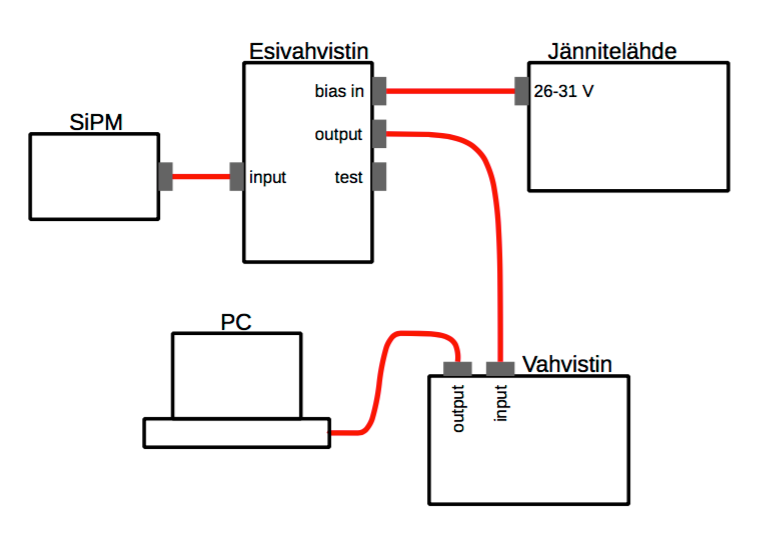
\includegraphics[scale=0.7]{Koejarjestely}
\label{fig:Koejarjestely}
\caption{Kaaviokuva koejärjestelystä. Jännitelähde tuotti 28V:n jännitettä.}
\end{figure}

Kuten mainittiin Johdannossa, tarkoituksena on että säteilylähteeltä tulevaa säteilyä osuu tuikeilmaisimeen ja muuttuu valoksi, jota voimistetaan valomonistinputkella (SiPM). Sen jälkeen signaali muutetaan sähköiseksi ja vahvistetaan (Esivahvistin ja vahvistin), jonka jälkeen se kulkeutuu tietokoneen äänikortin kautta PRA11-ohjelmalle.(PC)

\section{Teoria}

\section{Tulokset}

\section{Johtopäätökset}

\section{Viitteet}



\end{document}